
\documentclass[12pt]{report}
\usepackage[a4paper]{geometry}
\usepackage[myheadings]{fullpage}
\usepackage{fancyhdr}
\usepackage{lastpage}
\usepackage{graphicx, wrapfig, subcaption, setspace, booktabs}
\usepackage[T1]{fontenc}
\usepackage[font=small, labelfont=bf]{caption}
\usepackage{fourier}
\usepackage[protrusion=true, expansion=true]{microtype}
\usepackage[english]{babel}
\usepackage{sectsty}
\usepackage{url, lipsum}
\usepackage{xcolor}
\usepackage{listings}
\usepackage{spverbatim}
\usepackage{hyperref}


\renewcommand{\thesection}{\arabic{section}}
\setcounter{section}{0} %numeracija sekcija

\graphicspath{ {./images/} }
\setlength\parindent{0pt} %nemoj uvuci paragraph
\newcommand{\code}[1]{\texttt{#1}} % code u tekstu

%color
\definecolor{my_green}{rgb}{0.027, 0.663, 0.545}
\newcommand{\mygreen}[1]{{\color{my_green}#1}}
\definecolor{my_red}{rgb}{0.843, 0.000, 0.384}
\newcommand{\myred}[1]{{\color{my_red}#1}}


%---- CODE LISTING
\definecolor{codecomment}{rgb}{0.561, 0.561, 0.561}
\definecolor{codegray}{rgb}{0.5,0.5,0.5}
\definecolor{codepurple}{rgb}{0.58,0,0.82}
\definecolor{pozadina}{rgb}{0.925, 0.925, 0.925,}


\lstdefinestyle{mystyle}{
backgroundcolor=\color{pozadina},
commentstyle=\color{codecomment},
    keywordstyle=\color{magenta},
    numberstyle=\tiny\color{codegray},
    stringstyle=\color{codepurple},
	basicstyle=\ttfamily\footnotesize,
    breakatwhitespace=false,         
    breaklines=true,                 
    captionpos=b,                    
    keepspaces=true,                 
    numbers=left,                    
numbersep=3pt,
    showspaces=false,                
    showstringspaces=false,
    showtabs=false,                  
    tabsize=2
}
\lstset{style=mystyle}
%--------


\begin{document}

\newcommand{\HRule}[1]{\rule{\linewidth}{#1}}
\onehalfspacing


%-------------------------------------------------------------------------------
% HEADER & FOOTER
%-------------------------------------------------------------------------------
\pagestyle{fancy}
\fancyhf{}
\setlength\headheight{15pt}
\fancyhead[L]{CANAL PLUS}


%-------------------------------------------------------------------------------
% FIRST PAGE
%-------------------------------------------------------------------------------
\title{ \normalsize \textsc{CANAL PLUS}
\\ [1.0cm]
\HRule{0.5pt} \\
\LARGE \textbf{\uppercase{MAKE BUILDROOT}}
\HRule{2pt} \\ [0.5cm]
\normalsize  \vspace*{5\baselineskip}

\includegraphics[scale=0.8]{logo_rtrk.png}
}



\author{Miroslav Blazic}
\date{\today\\
\fbox {Version: v1.1}
}

\maketitle


%-------------------------------------------------------------------------------
% TABLE OF CONTENT
%-------------------------------------------------------------------------------
\newpage
\tableofcontents
\newpage



\section*{ABSTRACT}
This document contains instruction of make buildroot based on Ubuntu 12.04. \newline
The document is kept on the assumption that you already have corresponding linux OS.

\newpage



\section{INSTRUCTIONS}
\begin{center}
    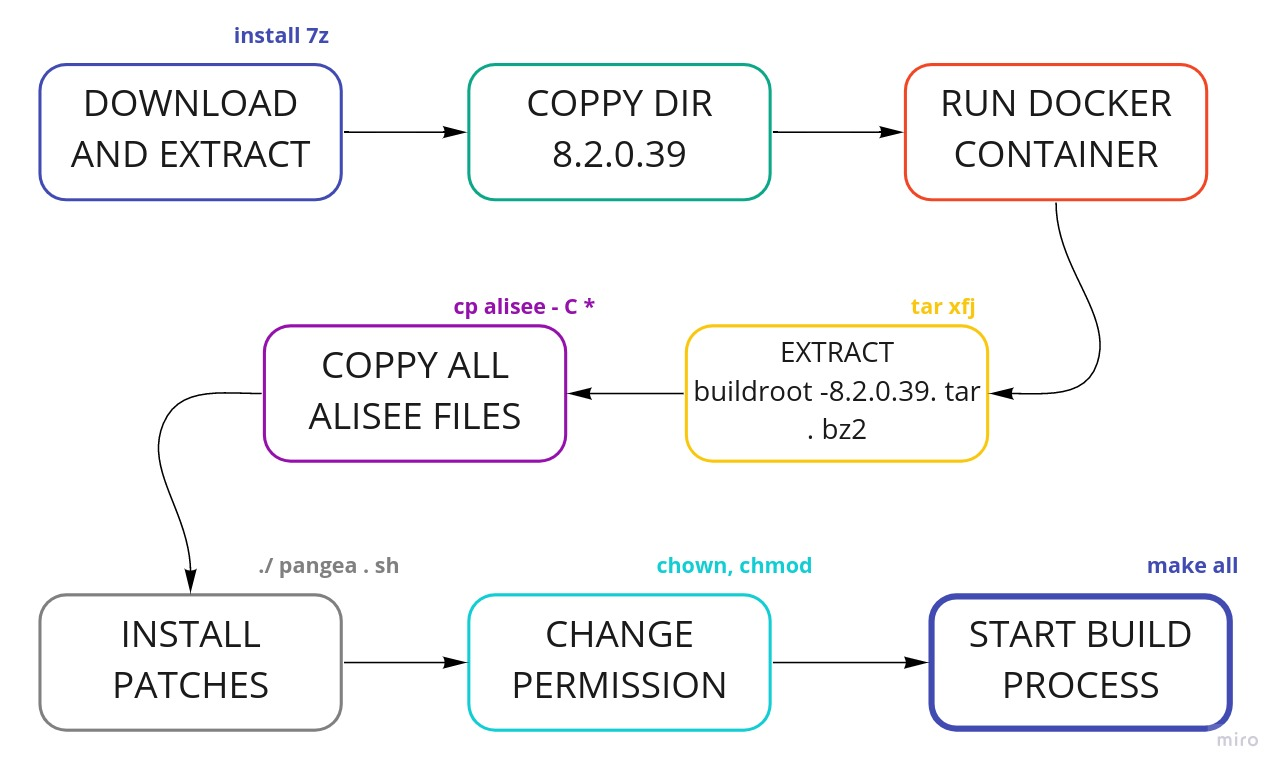
\includegraphics[scale=0.35]{make-buildroot.jpg}
\end{center}


\section{PREPARE DIRECTORIUM}
Firstly, we need to have a docker image \code{ali{\_}linux{\_}sdk.tar.gz} and dir \code{M3538.7z}.
You can download that from:
\begin{lstlisting}[caption= Download URL. ]
smb://samba03/proot/iwedia/Projects/113. Canal+/ALi/:
\end{lstlisting}

Create directorium \code{volume} which will use later as mount point with docker container,
and then extract \code{M3538.7z} file.
\begin{lstlisting}
mkdir -p ~/Desktop/volume
    7z x M3538.7z 
\end{lstlisting}

If you not have installed \code{7z}, follow the commands:
\begin{lstlisting}[language=C, caption= Install 7z. ]
    sudo apt-get update
    sudo apt-get install p7zip-full

    // check if it is installed 
    7z
\end{lstlisting}

Coppy dir 8.2.0.39 to dir volume

\begin{lstlisting}[language=C, caption= Coppy dir 8.2.0.39 ]
 cp -r <path>/M3538/M3538/iwedia/linux_sdk/8.2.0.39 ~/Desktop/volume

 // you can delete dir M3538 and M3538.7z
  rm -rf <path>/M3538
  rm -rf <path>/M3538.7z
\end{lstlisting}


\section{RUN DOCKER}
Downloaded docker image \code{ali{\_}linux{\_}sdk.tar.gz} should be import to docker:
\begin{lstlisting}[language=C, caption= Import docker image. ]
sudo docker load < ali_linux_sdk.tar.gz
\end{lstlisting}

After imported docker image should be make and run container from image:
\begin{lstlisting}[language=C, caption= Run docker container. ]
run -it --name <name-container> -v <path-to-extract-folder>:/data <image>:<version> /bin/bash

//example
run -it --name ali_sdk_container -v /home/user/Desktop/volume:/data ali_linux_sdk:latest /bin/bash

// Output should be as:
root@52d0dbd8e06d:/#

\end{lstlisting}
You should be there now in docker container and should can be to see dir 8.2.0.39:
\begin{lstlisting}[language=C, caption= Run docker container. ]
    ls /data
\end{lstlisting}

If you exited from container with command: \code{exit}, you can again enter to contaier with following commands:
\begin{lstlisting}[language=C, caption= Attach container. ]
    sudo docker start NAME_OF_CONTAINER
    sudo docker attach NAME_OF_CONTAINER
\end{lstlisting}



\section{MAKE BUILDROOT}
In docker container go to dir 8.2.0.39 and follow the commands:
\begin{lstlisting}[language=C]
cd /data/8.2.0.39
ls
// SDK_Change_List_8.2.0.39.xlsx                 apply-patches.sh
// SDK_Release_Note_8.2.0.39.xlsx                buildroot-8.2.0.39.tar.bz2
// alisee-C0100A-PDK3.2.0-20200609-Auto.tar.bz2  ca_docs
// alisee-C0101A-PDK3.2.0-20200609-Auto.tar.bz2  common_docs
// alisee-C0200A-PDK3.2.0-20200609-Auto.tar.bz2  mp_tools
// alisee-C1800A-PDK3.2.0-20200609-Auto.tar.bz2  pangea.sh
// alisee-C2000A-PDK3.2.0-20200609-Auto.tar.bz2  patches
// appendix_docs

// change owner and permission
chown nobody:nogroup . -R
chmod 777 -R .

\end{lstlisting}
Now should be extract\code{buildroot-8.2.0.39.tar.bz2} with options \code{tar xfj}.
\begin{lstlisting}[language=C]
tar xfj buildroot-8.2.0.39.tar.bz2
    
// again change owner and permission
chown nobody:nogroup . -R
chmod 777 -R .
\end{lstlisting}

Coppy all \code{alisee-C} files to dir \code{buildroot-8.2.0.39/release}:
\begin{lstlisting}[language=C]
cp alisee-C* buildroot-8.2.0.39/release/
\end{lstlisting}

Run shell script pangea.sh which will be install required patches:
\begin{lstlisting}[language=C]
    ./pangea.sh 

// Output should be:
// patching file package/shadow/shadow.mk

\end{lstlisting}


Run build process:
\begin{lstlisting}[language=C]
cd buildroot-8.2.0.39
    make clean
    make alim3538_ddk_c0200_nand_defconfig
    make all
\end{lstlisting}








\end{document}